\documentclass[letterpaper, 12pt]{article}
\usepackage[top=.5in,bottom=.5in,left=.75in,right=.75in,headheight=30pt, % as per the warning by fancyhdr
includehead,includefoot,
heightrounded, % to avoid spurious underfull messages
]{geometry}
\addtolength{\topmargin}{-.25in}
\usepackage{fancyhdr}
\pagestyle{fancy}
\usepackage{graphicx}
\usepackage{lastpage}
\usepackage{multicol}
\usepackage{xcolor}
\usepackage{gensymb}
\usepackage{xcolor}
\usepackage[makeroom]{cancel}

\begin{document}
\fancyhead[l]{	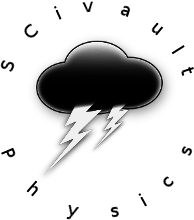
\includegraphics[height=0.5in]{../Logo/sp.png} Name: 
	\color{red} KEY - DO NOT REPRODUCE\color{black}}
\fancyhead[r]{Due Date: \hspace{ 1in}}
\fancyfoot[c]{\thepage\ of \pageref{LastPage}}
\fancyfoot[r]{Assignment 5.01}	


\begin{center} Assignment 5.01: Force
\end{center}
\vspace{-.3in}
\begin{enumerate}
\item A 600 kg car accelerates from 5 m/s to 10 m/s in three seconds.
\begin{enumerate}
	\item What is the acceleration of the car?
	
	\color{red}
	$a = \frac{v_f-v_i}{t} = \frac{10 m/s - 5 m/s} {3 s} \approx 1.667 m/s^2$
	
	\color{black}

	\item What is the force that the motor exerts on the car?
	
	\color{red}
	$F = ma = 600kg \cdot 1.667 m/s^2 \approx 360$N
	\color{black}


\end{enumerate}

\item Two children are playing tug-o-war.  Juan has a mass of 40 kg and pulls with a force of 20 N. Carlos has a mass of 20 kg and pulls with a force of 50 N.  
\begin{enumerate}
	\item Which way do the children go?
	\vspace{0.3in}
	\item What is the acceleration of the children?
	\vspace{0.4in}
	\item How far do they end up after 10 seconds?  
	\vspace{0.4in}
\end{enumerate}

\item  A pitcher throws a curve-ball at 20 m/s toward home plate, perfectly horizontal.  The ball leaves his hand 1.5 meters above the ground.  
\begin{enumerate}
	\item How far does the ball go?
	\vspace{0.4in}
	\item With what velocity (magnitude and direction) does the ball hit the ground?
	\vspace{0.4in}
\end{enumerate}


\item A car has a mass of 850 kg.  What is the weight of the car?
\vspace{0.4in}


\item A crane lifts a 1200 kg steel girder.  It causes the girder to accelerate at a rate of 0.2 m/s\textsuperscript{2} upward. 
\begin{enumerate}
	\item What force must the crane exert on the steel girder?
	\vspace{0.4in}
	\item How long does it take the crane to reach its top speed of 3 m/s?

\end{enumerate}

\pagebreak


\item You push a box across the floor with a force of 60 newtons for two seconds.  The force of friction on the box is 20 newtons.  The box has a mass of 40 kg.  
\begin{enumerate}
	\item What is the acceleration of the box?
	\vspace{0.4in}
	\item What is the speed of the box when you stop pushing it?
	\vspace{0.4in}
	\item What is the deceleration of the box when you stop pushing it?
	\vspace{0.4in}
	\item How long does it take the box to come to a complete stop?
	\vspace{0.4in}
	\item What is the final position of the box?
	\vspace{0.4in}
\end{enumerate}

\item A ball is dropped off a building.  At a certain time, it falls with an acceleration of 9.5 m/s\textsuperscript{2}. 
	\begin{enumerate}
		\item What is the net force acting on the ball at this time?
		\vspace{0.45in}		
		\item What is the force of gravity that is acting on the ball at this time?
		\vspace{0.45in}
		\item What is the force due to air resistance acting on the ball at this time?  
		\vspace{0.45in}
		\item At a later time, when the ball has fallen farther but has not yet hit the ground, is the magnitude of the net force on the ball greater than, less that, or equal to the net force in part (a)?  Justify your answer. 
		\end{enumerate}




\end{enumerate}


 



\end{document}
